%\documentclass{article}
\documentclass[fleqn,10pt,
paperheight=16cm, paperwidth=12cm,
includehead,% See below for an explanation
nomarginpar,% We don't want any margin paragraphs
textwidth=10cm,% Set \textwidth to 10cm
headheight=25pt,% Set \headheight to 2cm
%showframe % Show the page layout
]{wlscirep}


\usepackage{fancyhdr}
% 加上 table in the header 
% https://tex.stackexchange.com/questions/113240/tables-as-header-and-footer

\usepackage{hyperref} %加入 hyperlink

%\usepackage[utf8]{inputenc}
\usepackage[T1]{fontenc}
% https://www.overleaf.com/latex/examples/demonstration-of-noto-serif-cjk-and-noto-sans-cjk-fonts/sgrwgcddtqsq
\usepackage{setspace}

%set-up 中文環境
\usepackage[CJKspace]{xeCJK}
\usepackage{xpinyin}

\setmainfont{Noto Serif Light}
\setsansfont{Noto Sans}
\setmonofont[Scale=MatchLowercase]{Noto Mono}

\setCJKmainfont{Noto Serif CJK TC}
\setCJKsansfont{Noto Sans CJK TC}
\setCJKmonofont{Noto Sans Mono CJK TC}


%表格
\usepackage{amsmath}
\usepackage{amssymb}
\usepackage{hyperref}
\usepackage{array}

\usepackage{tabularx}
\usepackage{multirow}

\usepackage{ragged2e}
\usepackage{longtable}

\pagestyle{fancy}
\renewcommand{\headrulewidth}{1pt}
\fancyhead[CE,CO,LE,LO,RE,RO]{} %% clear out all headers
\fancyhead[L]{%

\includegraphics[width=\paperwidth/8]{images/general/fig_ntuh_logo.jpg}
新竹台大分院教學部 第 \thepage 頁/全部 \pageref{LastPage} 頁
}
%\fancyfoot[C]{第 \thepage 頁/全部 \pageref{LastPage}頁}




\begin{document}
\setlength{\headheight}{56.19998pt} %與 fancy有關，增加 header 的高度!


\title{
%
\includegraphics[width=\paperwidth/8]{images/general/fig_ntuh_logo.jpg}\\
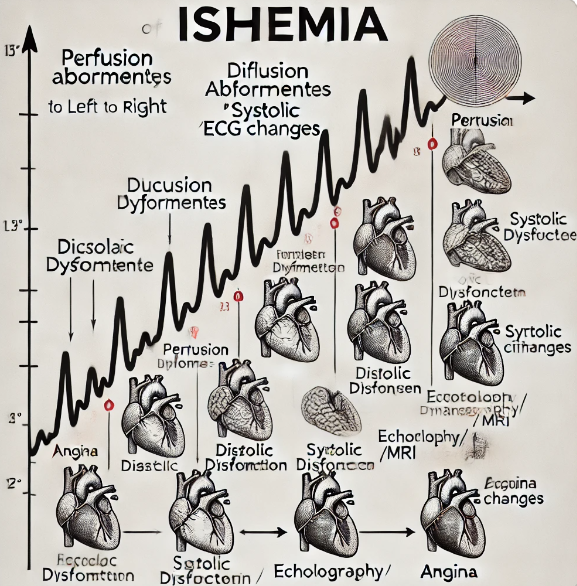
\includegraphics[width=0.80\paperwidth]{images/chest-pain/fig_chest_pain_logo.png}\\
\\
早期診斷心肌梗塞}
\author{謝慕揚醫師, Drake, NTUH Cardiology Fellow of 2009, Cardiovascular Center 2011-}
\date{}

\begin{abstract}
這是一個教學文件，指導醫院同仁如何早期辨識出心肌梗塞。
文章自2009開始編寫，期間內容以 Google Drive方式分享給同事們，在2024-09月以後開始以Latex型式編修。    
\end{abstract}

\maketitle

\tableofcontents


\onehalfspacing

\section{Early Diagnosis of Acute Myocardial Infarction- 前言}
\begin{itemize}
    \item 以前在intern時，讀過一本書，書名是Cope's Early Diagnosis of Acute Abdomen. 作者Zachary Cope在他的書中寫得很清楚，整本書跟evidence-based medicine無關，純粹是他個人診斷急性腹痛的經驗。全書他用栩栩如生的文字，將一個肚子痛的問診，理學檢查，以及診斷，洋洋灑灑寫了好幾萬字。讓讀的人有一個清楚的像貌，就算是沒真的接觸過perforate peptic ulcer, 也能在讀懂書之後，能夠有系統的處理，而不致於延誤診斷。這本書在經過Harvard Medical School的William Silen整理後，一直到現在還在出版。William Silen是唯一一個在Harrison's Internal Medicine有兩章是給外科醫師執筆的章節的作者。
    \item 現在當fellow了，在急診看過大大小小的AMI被delay診斷，不禁懷疑起一件事，為什麼書本都寫得清清楚楚的心肌梗塞的診斷方法，到了實際臨床要應用時，還是那麼困難？所有的胸痛，明明病人的症狀清楚，就因為對心電圖沒把握，所以一直要到cardiac enzymes高上去了，才能夠診斷AMI. 又或是常常cardiac enzymes因為顯而易見的原因而升高，但是因為lab data都列出來了，實在不容忽視，所以診斷又理所當然只剩下AMI, 而沒有其它的鑑別診斷了。
    \item 這份文件的目地只有一個，讓讀者對於心肌梗塞的病人，有一個清楚的輪廓，不要再在急診發生CV fellow到場，對於診斷過程跟處置，覺得不夠周延的場面了。
    \item 在evidence-based medicine跟guideline盛行的時代，有的時候，醫學的教育還是要訴諸經驗的傳承。所有的patient care不應該只照guideline處理，我想要強調的是：病患的照顧一定要individualized. 每個病人的表現都是unique的，前輩們的經驗，對照當代的evidence-based的研究，兩者合併，才是對的事。
\end{itemize}

\section{What Every Doctor Should Know}
\section*{Electrocardiography (心電圖)}

\subsection*{Principles- \textbf{Never hesitate to repeat ECG}}

當病人還在胸痛，還有症狀時，千萬要記得追蹤心電圖。如果是STEMI（ST elevation myocardial infarction），可以在短短的十五分鐘之內，由hyperacute T wave變成ST elevation。因此，如果第一張ECG是non-diagnostic（無法診斷），而病人又是持續性的胸痛（persistent pain），記得在十五分鐘之內再做一張ECG。千萬別等六小時再做，因為到時候可能已經出現QS pattern了。

心肌梗塞（myocardial infarction）的早期心電圖變化，以hyperacute T wave change最容易在急診第一時間被miss掉。2011-2015統計，所有被delay的STEMI當中，比例上，十張心電圖中，有七張都是因為沒有認出hyperacute T wave所致。另外要小心的是: 常常第一個看心電圖的醫師，只有看到reciprocal的ST depression，而忽略了其它lead可以見到的 ST elevation，以致於病人被當成NSTEMI治療（可是病患其實是STEMI!）。

\begin{figure}
    \centering
    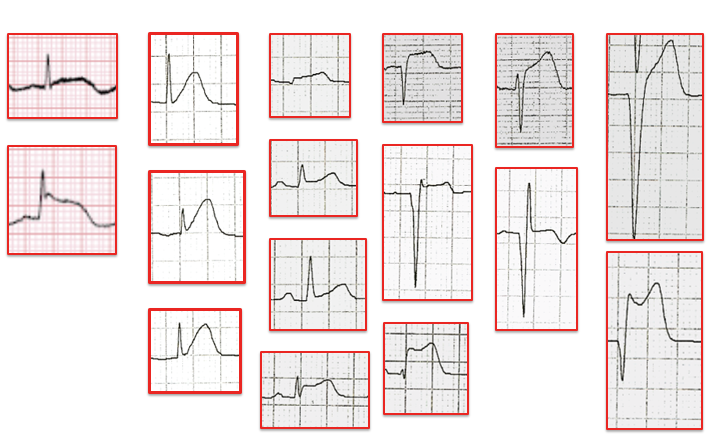
\includegraphics[width=\linewidth]{images/ecg/fig_ST_elevation_pattern.png}
    \caption{2011-2024年，新竹台大分院，各式ST elevation pattern圖譜。右邊的最好認，而越往左邊越難辨識。}
    \label{images/ecg/fig_ST_elevation_pattern}
\end{figure}


\section{ECG waveform interpretation- 波型辨識}
請先參考 Figure ~\ref{images/ecg/fig_ST_elevation_pattern}，這張圖裡面整理了2011-2024年新竹台大分院急診室，收集到的各式ST elevation pattern圖譜。右邊的最好認，而越往左邊越難辨識。

\begin{longtable}{p{4cm} p{9cm}}
\caption{ECG waveform recognition}\\
\hline
\textbf{項目} & \textbf{內容} \\
\hline
\endfirsthead
\multicolumn{2}{l}{\textit{接續上一頁}} \\
\hline
\textbf{項目} & \textbf{內容} \\
\hline
\endhead
\hline \multicolumn{2}{r}{\textit{接續下一頁}} \\
\endfoot
\endlastfoot

\textbf{Hyperacute T wave} & 
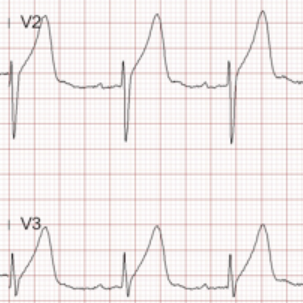
\includegraphics[width=0.9\linewidth]{images/ecg/fig_ST_elevation_hyperacute T.png}
這是hyperacute T wave的ECG, T wave很高，高得比R wave還高。同時可以見到ST segment明顯地拉上去了 (ST elevation). 

\\ \hline

\textbf{ST elevation} & 
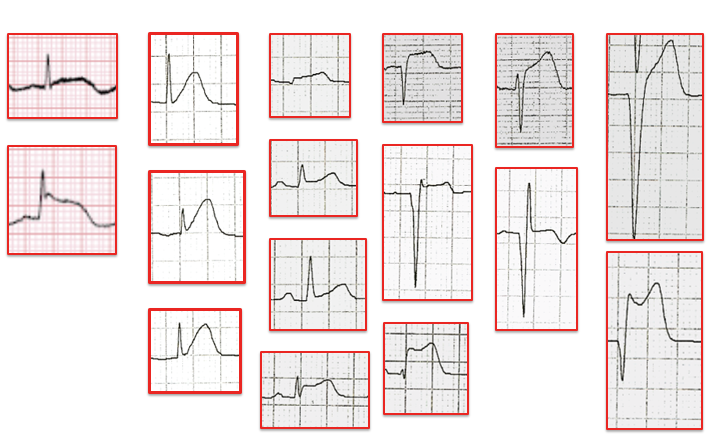
\includegraphics[width=0.9\linewidth]{images/ecg/fig_ST_elevation_pattern.png}



請另外參考 Figure ~\ref{images/ecg/fig_ST_elevation_pattern}. \\

& 
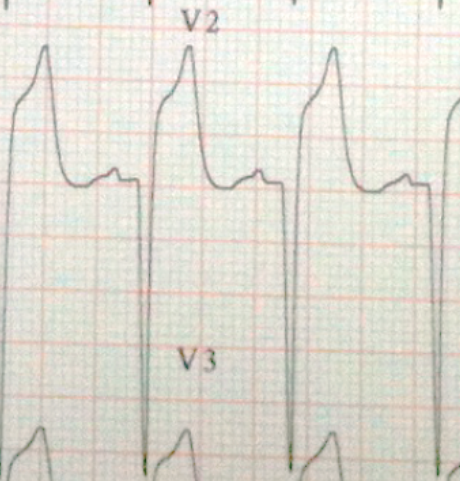
\includegraphics[width=0.5\linewidth]{images/ecg/fig_ST_elevation_1.png}


在V2-3, QS都已經出來了，同時ST elevation也很明顯，這時的T wave還是upright. 另外可以見到的是: sinus tachycardia, 有個P wave在QS pattern之前。 \\

& 
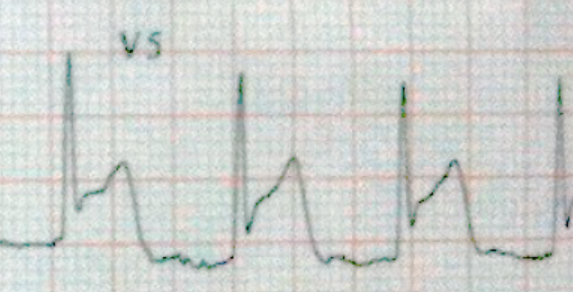
\includegraphics[width=0.5\linewidth]{images/ecg/fig_ST_elevation_2.png}


在V5還有R wave, 同時是很明顯的ST elevation, 跟上例一樣，如果連續兩個leads都有見到，那馬上就可以聯絡急導管了。按照經驗，這麼明確而且高的ST elevation, 一定是在相鄰的好幾個leads都見得到STE, 同時在其它導程，也會見到明顯的reciprocal change. 

\\ \hline

\textbf{QS pattern with ST elevation} & 
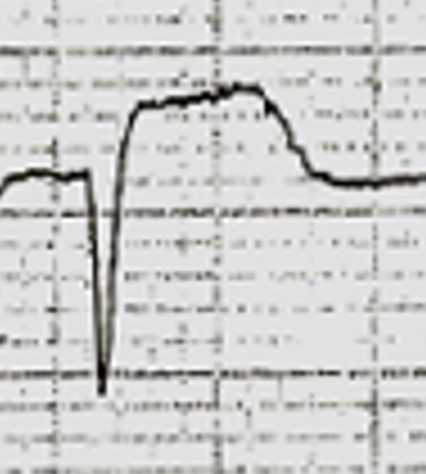
\includegraphics[width=0.5\linewidth]{images/ecg/fig_ST_elevation_QS.png}
\\ \hline

\textbf{T wave inversion} & 
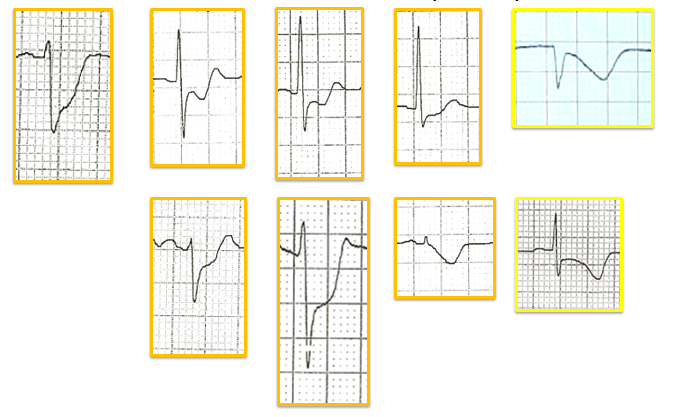
\includegraphics[width=0.9\linewidth]{images/ecg/fig_ST_depression_TWI.png}

\\ \hline
\end{longtable}

\section{病史詢問與理學檢查- A timely approach 評估應該要注意時效}

\begin{longtable}{p{4cm} p{9cm}}
\caption{胸痛病史詢問與鑑別診斷}\\
\hline
\textbf{項目} & \textbf{內容} \\
\hline
\endfirsthead
\multicolumn{2}{l}{\textit{接續上一頁}} \\
\hline
\textbf{項目} & \textbf{內容} \\
\hline
\endhead
\hline \multicolumn{2}{r}{\textit{接續下一頁}} \\
\endfoot
\endlastfoot

\textbf{胸痛病史詢問} & 
當第一時間知道病人有胸痛時，不論如何（不管胸痛多嚴重，或當時有其它任何complaint）都馬上立刻做一張心電圖。心電圖不應該有任何delay的理由。確定有人開始做心電圖之後，馬上跟病患的陪同者確認病史。待病患完成心電圖後，再把重要的訊息做確認，根據心電圖的發現，儘快做治療的決定。\\ \hline

\textbf{STEMI病史詢問} & 
病患常常除了胸痛之外，還會有全身性的主訴，像是覺得累，容易疲倦（malaise, frank exhaustion）。胸痛的性質也會不太一樣，有的老人家只講悶（結果做起來是LAD proximal total occlusion!），有的則是很痛很痛（intolerable pain）。胸痛的嚴重程度在STEMI時，當然是較嚴重，同時持續的時間也長（超過30分鐘，有的則長到好幾個小時都在痛）。

胸痛的病史詢問，務必記得要問 pain scale! 阿伯，請您現在跟我評分一下胸痛的指數是多少? 0分是不痛，1分是很輕的痛，10分是痛到受不了。請務必讓病人口述疼痛指數，不要只憑外觀表現幫病人評胸痛指數。當然如果病人已經插管，或是意識障礙，不然都應該要評疼痛指數。請注意，在急性冠心症的病患，評估不應該造成處置的延遲。

\\ \hline

\textbf{胸痛的形容} & 
各式各樣形容chest pain的詞語：緊緊的（constricting）, crushing, oppressing, compressing, heavy weight, squeezing, 偶爾也會有atypical的詞：choking, viselike, stabbing, knifelike, boring, burning。痛的radiation典型的是痛到下巴，痛到雙肩，延著左前臂到手指，也會有只痛喉嚨或手腕的表現。\\ \hline

\textbf{STEMI vs. Angina} & 
STEMI的痛通常會比unstable angina, stable angina來得更厲害，持續的時間更久，且對NTG無反應。


拜託千萬不要再發生下面的推理敘述: "因為病患的疼痛對於NTG反應很差，所以應該不是STEMI。" (這是完全錯誤的推論性敘述。\\ \hline

\textbf{無痛STEMI} & 
在某些族群如elderly, women, diabetic patients, heart transplant patients，STEMI可能表現為胸悶、心衰、交感神經過度活化，而非典型的胸痛症狀。\\ \hline

\textbf{症狀誤診} & 
inferior wall MI常表現為nausea/vomiting，容易被誤診為急性膽囊炎、消化性潰瘍、胃炎等。\\ \hline

\textbf{其它症狀} & 
profound weakness, dizziness, palpitations, cold perspiration, sense of impending doom。\\ \hline

\textbf{藥物史詢問} & 
現在服用什麼藥？是否每天服用aspirin？是否有服用威而鋼？這些將決定治療決策。\\ \hline

\textbf{鑑別診斷} & 
發燒、畏寒、發抖寒顫、咳痰、頻尿等症狀的詢問可以幫助排除其他診斷。\\ \hline

\end{longtable}


\section{病歷調閱}
\begin{longtable}{p{4cm} p{9cm}}
\caption{病患住院病摘及心電圖資料檢視}\\
\hline
\textbf{項目} & \textbf{內容} \\
\hline
\endfirsthead
\multicolumn{2}{l}{\textit{接續上一頁}} \\
\hline
\textbf{項目} & \textbf{內容} \\
\hline
\endhead
\hline \multicolumn{2}{r}{\textit{接續下一頁}} \\
\endfoot
\endlastfoot

\textbf{Chart} & 
病患之前的住院病摘要快速調閱，內容包括:
\begin{itemize}
    \item 何時做的心導管？
    \item 幾條血管被involve？
    \item 放的是什麼支架？
    \item 以及有無合併其他共病（co-morbidity）如cancer, hypertension, diabetes mellitus, dyslipidemia？
\end{itemize}
\\ \hline

\textbf{ECG} & 心電圖可以在電腦系統中取得，所有團隊成員都必要要能夠熟悉電子病歷如何調閱心電圖。\\ \hline

\textbf{舊ECG的比較} & 什麼時候需要立刻跟舊的ECG做比較？需要知道病患的LBBB是否是舊的，是否早已有QS pattern with ST elevation（with apical aneurysm formation）。 \\ \hline

\textbf{心臟超音波 (echocardiography)} & 如果病患之前做過心臟超音波，可以立即檢查LVEF（心臟收縮功能）及LVEDD（心臟是否擴大），並檢查有無valvular heart disease。重點應放在LVEF, LVEDD, MR或AR。 \\ \hline

\end{longtable}

\section{第一張心電圖看不出問題!}

\begin{longtable}{p{4cm} p{9cm}}
\caption{Negative ECG at First Scene與風險因子分析}\\
\hline
\textbf{項目} & \textbf{內容} \\
\hline
\endfirsthead
\multicolumn{2}{l}{\textit{接續上一頁}} \\
\hline
\textbf{項目} & \textbf{內容} \\
\hline
\endhead
\hline \multicolumn{2}{r}{\textit{接續下一頁}} \\
\endfoot
\endlastfoot

\textbf{Negative ECG at First Scene} & 
常常第一張心電圖是無法診斷的，這時請還是重視病患的臨床症狀和徵象。如果是明顯厲害的胸痛，仍然可以當作ACS或unstable angina來治療。接下來要繼續完成病史詢問。 \\ \hline

\textbf{Risk factors} & 
當不需要緊急進行心導管時，應花時間釐清風險因子。\\ \hline

\textbf{風險因子} & 
\begin{itemize}
    \item 年齡 (Age)
    \item 冠狀動脈疾病史 (History of CAD)
    \item 男性 (Male gender)
    \item 吸菸者 (Active smoker)
    \item 糖尿病 (Diabetes mellitus)
    \item 血脂異常 (Dyslipidemia)
    \item 家族冠狀動脈疾病或AMI史 (Family history of CAD/AMI)
\end{itemize} \\ \hline

\textbf{風險因子缺乏的情況} & 
即使患者沒有任何風險因子，仍不能因此排除心肌缺血，仍應依臨床證據為主。\\ \hline

\textbf{年輕患者發生AMI的情況} & 
以下幾種情況應特別鑑別，因其可能導致年輕患者發生AMI：
\begin{itemize}
    \item 冠狀動脈先天異常 (Coronary congenital anomaly)
    \item 童年患川崎病伴冠狀動脈瘤 (Kawasaki disease in childhood with coronary aneurysm)
    \item 產後女性 (Female in post-partum status)
    \item 可卡因或其他藥物成癮 (Cocaine use or other drug addiction)
    \item 嗜鉻細胞瘤 (Pheochromocytoma)
    \item 感染性心內膜炎導致冠狀動脈栓塞 (Coronary emboli from infective endocarditis)
\end{itemize} \\

\hline
\end{longtable}


\section{共病的確認}
\begin{longtable}{p{4cm} p{9cm}}
\caption{合併症鑑別診斷與處理}\\
\hline
\textbf{項目} & \textbf{內容} \\
\hline
\endfirsthead
\multicolumn{2}{l}{\textit{接續上一頁}} \\
\hline
\textbf{項目} & \textbf{內容} \\
\hline
\endhead
\hline \multicolumn{2}{r}{\textit{接續下一頁}} \\
\endfoot
\endlastfoot

\textbf{Comorbidity identification} & 
病患的胸痛屬實，第一個還是要考慮心肌缺血 (myocardial ischemia)。以下是最重要的AMI鑑別診斷及合併症 (comorbidity)：
\begin{itemize}
    \item 主動脈剝離 (Aortic dissection)
    \item 肺栓塞 (Pulmonary embolism)
    \item 心包炎 (Pericarditis)
    \item 敗血症 (Sepsis)
\end{itemize} \\ \hline

\textbf{Sepsis patients} & 
對於sepsis的病人，不應魯莽地進行急導管檢查，這常會讓病患的病情更加惡化。 
試想一個sepsis合併DIC、多器官衰竭（包括急性腎衰竭）的病人，如果進行導管檢查，接受大量造影劑的暴露，再放置支架並使用heparin，可能導致更加嚴重的後果。敗血症引起的心肌抑制通常是可逆的，通過正確的抗生素治療和足夠的支持性管理（如呼吸機、CVVH支持，有時甚至需要IABP），病情有可能逆轉。\\ \hline

\textbf{鑑別診斷: Cardiogenic shock vs. Septic shock} & 
在許多情況下，無需依靠導管診斷即可鑑別心源性休克和敗血性休克。我們應依據臨床表現及相關檢查來做出診斷。\\ \hline

\textbf{Elevated Troponin-I 鑑別診斷} & 
如果病人Troponin-I升高，需謹慎鑑別原因，重要的鑑別診斷包括：
\begin{itemize}
    \item 心肌梗塞 (Myocardial infarction)
    \item 敗血症 (Sepsis)
    \item 肺栓塞 (Pulmonary embolism)
    \item 腎功能不全 (Renal insufficiency)
    \item 一過性心室上性心搏過速 (Transient supraventricular tachycardia)
    \item CPR後或電擊後 (Post CPR/DC shock)
    \item 胃腸道出血 (GI bleeding)
\end{itemize} 
\\ \hline

\textbf{GI bleeding and PCI} & 
有些AMI病人的問題不是因為延遲進行PCI，而是由於胃腸道出血造成的繼發性心肌缺血。導管手術成功或失敗的同時，病人在CCU中可能會出現難以控制的GI出血。這些病人因為已經放置了支架並使用了heparin，導致GI出血無法止住，最終可能因出血而死亡。導管雖然成功，但病人卻因此喪命，這是非常令人遺憾的情況。\\ \hline

\textbf{病史詢問 (Hx)} & 
最近三天有沒有解黑便（tarry stool）？有沒有消化性潰瘍病史、GERD，或者曾經進行過腹部手術？\\ \hline

\textbf{理學檢查 (PE)} & 
檢查病人的結膜是否蒼白（pale conjunctivae）、手掌是否蒼白（pale palm）、嘴唇是否蒼白（pale lips）？這些基本的檢查可以幫助決定是否需要進行直腸指診（digital anal exam）。\\ \hline

\textbf{治療 (Tx)} & 
如果上消化道出血的證據確鑿，請勿給予aspirin或heparin。應先糾正貧血。如果病人同時有嚴重的胸痛，則應直接使用抗血小板藥物（如clopidogrel）和抗心絞痛藥物（如NTG）。至於是否使用aspirin、heparin或進行PCI，需由心臟科醫師決定。\\ \hline

\end{longtable}

\section{理學檢查}

\begin{longtable}{p{4cm} p{9cm}}
\caption{STEMI患者的理學檢查}\\
\hline
\textbf{項目} & \textbf{內容} \\
\hline
\endfirsthead
\multicolumn{2}{l}{\textit{接續上一頁}} \\
\hline
\textbf{項目} & \textbf{內容} \\
\hline
\endhead
\hline \multicolumn{2}{r}{\textit{接續下一頁}} \\
\endfoot
\endlastfoot

\textbf{Physical examination (理學檢查)} & STEMI病人的理學檢查應關注於其外觀和徵象，這些可幫助判斷病情的嚴重程度。 \\ \hline

\textbf{General appearance of STEMI} & STEMI病人（或其他重症病人）通常會顯得焦慮緊張（anxious），並表現出極度的痛苦或不適（in considerable distress）。病人通常會不安地在床上扭動（restless），相較之下，單純的心絞痛（angina）病人會比較平靜，因為他們知道任何動作都可能加重胸痛。STEMI病人幾乎找不到一個舒服的姿勢。 \\ \hline

\textbf{胸部動作與Levine's sign} & 病人可能會不自覺地按摩或捶打自己的胸部（massage or clutch their chests），經常在胸口上做出握拳動作（clenched fist over chest），這是表達疼痛的典型動作（Levine's sign, named after Dr. Samuel A. Levine）。 \\ \hline

\textbf{LV dysfunction徵象} & 如果病人有左心室功能不全（LV dysfunction），因交感神經刺激（sympathetic stimulation），會伴隨盜汗（cold perspiration）和臉色蒼白（skin pallor）。病人的呼吸模式也會改變，這通常是由於肺部充血和水腫（lung congestion and edema）的進展所致，因此病人可能會坐在床邊張口喘氣（gasping）。很多中年男性會描述喉嚨緊繃，像是被掐住一般，感到呼吸困難（feeling of suffocation）。 \\ \hline

\textbf{咳嗽與肺水腫} & 如果病人開始狂咳，或咳出粉紅色泡沫痰（pink frothy sputum），這往往代表病情已經進展到明顯的肺水腫（frank lung edema）。 \\ \hline

\textbf{Cardiogenic shock徵象} & 當病人進入心源性休克狀態（cardiogenic shock status）時，病人通常會一動不動地躺在床上（listless or lethargic）。其皮膚看起來非常蒼白（pallor），並且摸起來冰冷潮濕（cold and clammy）。四肢可能出現斑紋狀紋路（mottling），呈現藍或白色。四肢、指甲床及嘴唇可能出現發紺（cyanosis）。 \\ \hline

\textbf{CNS方面徵象} & 隨著休克的嚴重程度進展，病人可能會變得意識模糊或混亂（disoriented and confusion）。 \\ \hline

\textbf{Severe shock表現} & 這些表現通常見於重度休克的病人。有時候，即使病人血壓並未降低，依然可以處於休克狀態（normotensive shock）。因此，不應僅依據血壓做臨床判斷，而應根據病人的其他嚴重徵象來做出診斷和治療計劃。 \\ \hline

\end{longtable}

\newpage
\section{冠狀動脈血管攝影 Primer}

\begin{longtable}{p{4cm} p{9cm}}
\caption{Coronary angiography primer}\\
\hline
\textbf{項目} & \textbf{內容} \\
\hline
\endfirsthead
\multicolumn{2}{l}{\textit{接續上一頁}} \\
\hline
\textbf{項目} & \textbf{內容} \\
\hline
\endhead
\hline \multicolumn{2}{r}{\textit{接續下一頁}} \\
\endfoot
\endlastfoot

\textbf{Left coronary artery, LCA} & 
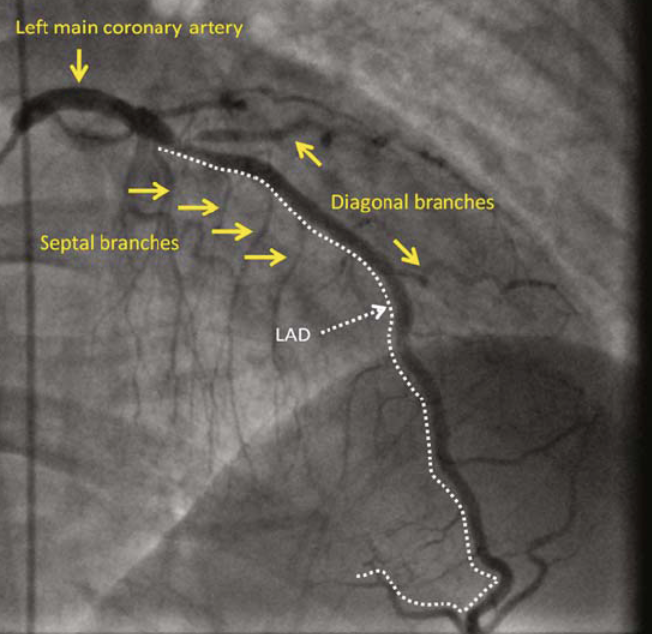
\includegraphics[width=0.9\linewidth]{images/angio/fig_angio_LCA 1.png}
\\ \hline

\textbf{Left coronary artery, LCA, RAO CAUDAL view} & 
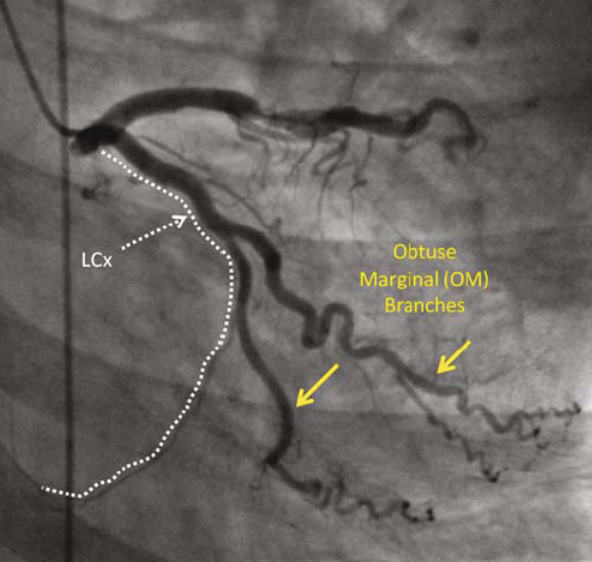
\includegraphics[width=0.9\linewidth]{images/angio/fig_angio_LCA 2.png}
\\ \hline

\textbf{Right coronary artery, RCA} & 
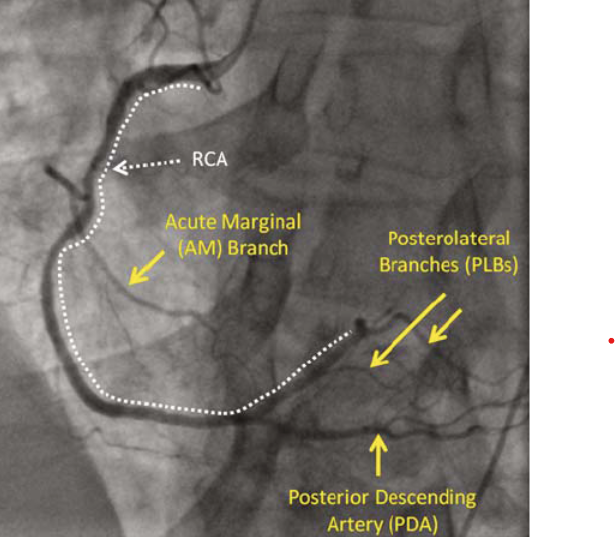
\includegraphics[width=0.9\linewidth]{images/angio/fig_angio_RCA.png}
\\ \hline
\end{longtable}



\end{document}
